\subsection{Теорема о вложенных отрезках}
\begin{theorem-non}
    \quad \\
    Если $[a_1, b_1] \supset [a_2, b_2] \supset [a_3, b_3] \supset \dots$ \\
    То $\exists c\in \R : c \in [a_n, b_n] \forall n \in \N$
\end{theorem-non}
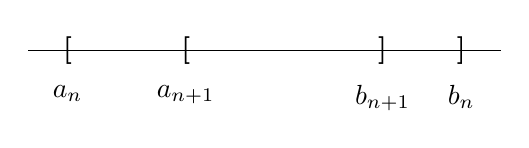
\begin{tikzpicture}
    \draw (-.5,0)--(5.5,0);
    \draw[color=black] (0, 0) node {\bfseries[} node[below=9pt]{$a_{n}$};
    \draw[color=black] (5, 0) node {\bfseries]} node[below=9pt]{$b_{n}$};
    \draw[color=black] (1.5, 0) node {\bfseries[} node[below=9pt]{$a_{n+1}$};
    \draw[color=black] (4, 0) node {\bfseries]} node[below=9pt]{$b_{n+1}$};
\end{tikzpicture}
\begin{proof}
    \quad \\
    $A = \{a_1, a_2, a_3, \dots\} \\
    B = \{b_1, b_2, b_3, \dots\} \\
    a_i \leqslant b_j, \forall i,j \in \N \\
    \forall i \leqslant j : a_i \leqslant a_j \leqslant b_j \leqslant b_i, \forall i \geqslant j : a_i \geqslant a_j \geqslant b_j \geqslant b_i$ \\
    По аксиоме полноты $\forall i, j \in \N \; \exists c \in \R: a_i \leqslant c \leqslant b_j \Longrightarrow \forall i \in \N : a_i \leqslant c \leqslant b_i$ \\
\end{proof}
\notice
\begin{enumerate}
    \item Теорема неверна для полуинтервалов \\
    Пример: $\bigcap\limits_{n = 1}^{\infty}(0; {{1}\over{n}}] = \varnothing$
    \item Теорема неверна для лучей \\
    Пример: $\bigcap\limits_{n = 1}^{\infty}(n; +\infty) = \varnothing$
    \item Теорема неверна без аксиомы полноты \\
    Пример: число $\pi$ \\
    $[3;\; 4] \supset [3,1;\; 3,2] \supset [3,14;\; 3,15] \supset \dots$ \\
    Пересечение не содержит рациональных чисел
\end{enumerate}